\section{Baseline and Fusion Results}
\subsection{Unimodal Baselines (v4 protocol)}
Table~\ref{tab:unimodal} reproduces the v4 unimodal baselines. \revnote{These were computed by 10-fold CV \emph{on the SMOTE-balanced training partition}, so synthetic patients appear in the test folds and the scores are optimistic (Section~VI-D quantifies this bias). Leak-free values under the controlled protocol are given in Table~\ref{tab:e1}: the clinical-only soft-voting system reaches AUC \clinAUC{} \clinAUCci{}, and clinical-only logistic regression without any resampling reaches \clinLRAUCval{}.} ECG-only scores use PTB-XL labels and are not comparable with Cleveland scores (Section~III-C).

\begin{table}[!t]
\centering\scriptsize
\caption{Unimodal baselines from v4 (10-fold CV on the SMOTE-balanced training partition; optimistic, see text).}
\label{tab:unimodal}
\setlength{\tabcolsep}{2.5pt}
\begin{tabular}{llccccc}
\toprule
Data & Model & Acc. & AUC & F1 & Prec. & Rec.\\
\midrule
Clinical & Logistic regression & 0.832 & 0.894 & 0.830 & 0.849 & 0.818\\
Clinical & SVM (RBF) & 0.817 & 0.889 & 0.808 & 0.857 & 0.771\\
Clinical & Random forest & 0.813 & 0.904 & 0.810 & 0.835 & 0.793\\
Clinical & XGBoost & 0.809 & 0.882 & 0.812 & 0.815 & 0.817\\
\midrule
ECG (PTB-XL) & Logistic regression & 0.797 & 0.871 & 0.781 & 0.845 & 0.730\\
ECG (PTB-XL) & SVM (RBF) & 0.824 & 0.910 & 0.820 & 0.823 & 0.826\\
ECG (PTB-XL) & Random forest & 0.831 & 0.912 & 0.823 & 0.849 & 0.807\\
ECG (PTB-XL) & XGBoost & 0.790 & 0.898 & 0.773 & 0.828 & 0.737\\
\bottomrule
\end{tabular}
\end{table}

\subsection{Fusion Results Reported in v4}
Table~\ref{tab:v4fusion} lists the v4 fusion results \emph{with their actual protocols}. The v4 table presented all rows as hold-out results. In fact the first four rows were CV means on the SMOTE-balanced training partition, and the ``MCF-BiModNet XGB'' and ``Soft-Voting'' rows were the same soft-voting model. On the seed-42 hold-out the soft-voting model correctly identified 26 of 28 CAD patients and 28 of 33 non-CAD patients (Fig.~\ref{fig:eval}).

\begin{table}[!t]
\centering\scriptsize
\caption{v4 fusion results with corrected protocol labels.}
\label{tab:v4fusion}
\setlength{\tabcolsep}{2.5pt}
\begin{tabular}{lcccc}
\toprule
Model & Protocol & Acc. & AUC & Rec.\\
\midrule
Feature fusion -- RF & CV, SMOTE train set & 0.794 & 0.869 & 0.756\\
Feature fusion -- XGB & CV, SMOTE train set & 0.809 & 0.877 & 0.824\\
Soft voting (untuned) & CV, SMOTE train set & 0.821 & 0.891 & 0.801\\
Stacking & CV, SMOTE train set & 0.829 & 0.894 & 0.817\\
Clinical MLP (labelled ``DL dual-branch'') & hold-out (61) & 0.803 & 0.882 & 0.786\\
Tuned soft voting (``MCF-BiModNet'') & hold-out (61) & 0.885 & 0.954 & 0.929\\
\midrule
Tuned soft voting, fused & 10-fold CV (303) & 0.815 & -- & --\\
Tuned XGB, clinical vs.\ fused & 10-fold CV (303) & 0.815 vs.\ 0.815 & -- & --\\
\bottomrule
\end{tabular}
\end{table}

\begin{figure}[!t]
\centering
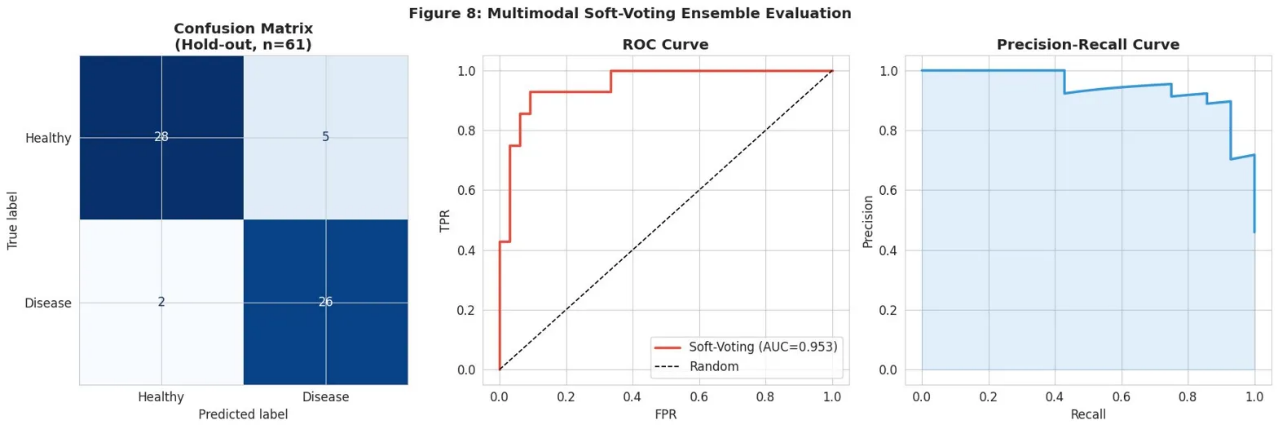
\includegraphics[width=\linewidth]{fig3_evaluation.png}
\caption{v4 soft-voting model on the seed-42 hold-out: confusion matrix, ROC and precision--recall curves. Section~VI-D shows that this split is unusually favourable.}
\label{fig:eval}
\end{figure}

\subsection{What the v4 Numbers Do and Do Not Show}
The v4 manuscript reported a ``+7.04 pp'' fusion gain. It was computed as the fused model's \emph{hold-out} accuracy (0.8852) minus the clinical XGBoost's \emph{10-fold CV} accuracy (0.8148), two numbers obtained under different protocols. Under the same protocol the v4 notebook itself found identical CV accuracy for clinical and fused XGBoost (0.8148 vs.\ 0.8148; paired $t=0$, $p=1.00$; McNemar $\chi^2=0.125$, $p=0.72$). Section~VI re-examines this and every other component claim under one controlled protocol.
